\documentclass{article}
\usepackage{styles}

\title{Image Processing\\
    Lab 4}
\author{Kevin Gevers (s25595987) \\ Jeroen Overschie (s2995697)\\Group 01}
\date{\today}

\begin{document}

\maketitle

Note, that all used source code can be found attached next to this report's pdf file. Its structure should be self-explanatory; all requested functions are named accordingly and any extra functions are explained in the report. Note that (almost) every function has a corresponding test script, which is named just like its function, but with a suffix '\texttt{\_test}'. Where possible, we followed the terminology from the book \citep{gonzalez2008digital} for variable naming.

\section*{Exercise 1}
In this first exercise, we are asked to solve Problem 9.9 from the book, from the Morphological Image Processing chapter. The exercise entails sketching dilations and erosions from some (binary) set using various Structuring Elements (SE's). Let us first illustrate the set $A$ on which the morphological operations will be applied on, and the respective Structuring Elements, $B^1$, $B^2$, $B^3$ and $B^4$.

\begin{figure}[H]
     \centering
     \begin{subfigure}[b]{0.3\textwidth}
         \centering
         \includesvg[width=\textwidth]{Assignment_4/pen&paper/A.svg}
         \caption{The input set $A$.}
         \label{fig:set_A}
     \end{subfigure}
     \hfill
     \begin{subfigure}[b]{0.08\textwidth}
         \centering
         \includesvg[width=\textwidth]{Assignment_4/pen&paper/B1.svg}
         \caption{$B^1$}
         \label{fig:SE_B1}
     \end{subfigure}
     \hfill
     \begin{subfigure}[b]{0.15\textwidth}
         \centering
         \includesvg[width=\textwidth]{Assignment_4/pen&paper/B2.svg}
         \caption{$B^2$}
         \label{fig:SE_B2}
     \end{subfigure}
     \hfill
     \begin{subfigure}[b]{0.11\textwidth}
         \centering
         \includesvg[width=\textwidth]{Assignment_4/pen&paper/B3.svg}
         \caption{$B^3$}
         \label{fig:SE_B3}
     \end{subfigure}
     \hfill
     \begin{subfigure}[b]{0.18\textwidth}
         \centering
         \includesvg[width=\textwidth]{Assignment_4/pen&paper/B4.svg}
         \caption{$B^4$}
         \label{fig:SE_B4}
     \end{subfigure}
     
    \caption{An overview of the Structuring Elements $B^1 ... B^4$ to be used in Exercise 1, along with its input set, $A$.}
    \label{fig:ex1_overview}
\end{figure}

A notable observation is that, for the Structuring Elements, it is not always the case that the origin lies in the middle of the shape. For most, the origin is indeed in the shape center, but for $B^3$ (see Figure~\ref{fig:SE_B3}) the origin is at the bottom-right point of the shape. This is important to note since it has an effect on the dilation/erosion procedures. For the other shapes, the origin lies at the center point.

\subsection*{(a)} In the first assignment, we first erode A by $B^4$ and then dilate the result by $B^2$, i.e. $(A \ominus B^4) \oplus B^2$. The result of the operation can be seen in Figure~\ref{fig:ex1_a}.

\begin{figure}[H]
     \centering
     \begin{subfigure}[b]{0.3\textwidth}
         \centering
         \includesvg[width=\textwidth]{Assignment_4/pen&paper/A.svg}
         \caption{The input set $A$.}
         \label{fig:ex1_a-inputset}
     \end{subfigure}
     \hfill
     \begin{subfigure}[b]{0.3\textwidth}
         \centering
         \includesvg[width=\textwidth]{Assignment_4/pen&paper/(a)-step1.svg}
         \caption{$(A \ominus B^4)$}
         \label{fig:ex1_a-step1}
     \end{subfigure}
     \hfill
     \begin{subfigure}[b]{0.3\textwidth}
         \centering
         \includesvg[width=\textwidth]{Assignment_4/pen&paper/(a)-step2.svg}
         \caption{$(A \ominus B^4) \oplus B^2$}
         \label{fig:ex1_a-step2}
     \end{subfigure}
     
    \caption{Overview of the erosion and dilation of assignment (a), using the SE's $B^4$ (Figure~\ref{fig:SE_B4}) and $B^2$ (Figure~\ref{fig:SE_B2}).}
    \label{fig:ex1_a}
\end{figure}

It can be observed that the first erosion strips off almost all foreground pixels. The circle shape only fits a very select amount of pixels, leaving out only what looks like the 'skeleton' of the original cross shape. In fact, since the circle is of diameter $L$, meaning it can 'perfectly' fit the sections of the cross, it can be seen as a \textit{maximum disk} for $A$. In the following dilation operation, many foreground pixels are added around the cross shape, and including some interesting looking 'tips' at the end of the cross points.

\subsection*{(b)} Next, we erode by $B^1$ and then dilate by $B^3$, i.e. $(A \ominus B^1) \oplus B^3$. The result of this operation can be seen in Figure~\ref{fig:ex1_b}.

\begin{figure}[H]
     \centering
     \begin{subfigure}[b]{0.28\textwidth}
         \centering
         \includesvg[width=\textwidth]{Assignment_4/pen&paper/A.svg}
         \caption{The input set $A$.}
         \label{fig:ex1_b-inputset}
     \end{subfigure}
     \hfill
     \begin{subfigure}[b]{0.29\textwidth}
         \centering
         \includesvg[width=\textwidth]{Assignment_4/pen&paper/(b)-step1.svg}
         \caption{$(A \ominus B^1)$}
         \label{fig:ex1_b-step1}
     \end{subfigure}
     \hfill
     \begin{subfigure}[b]{0.37\textwidth}
         \centering
         \includesvg[width=\textwidth]{Assignment_4/pen&paper/(b)-step2.svg}
         \caption{$(A \ominus B^1) \oplus B^3$}
         \label{fig:ex1_b-step2}
     \end{subfigure}
     
    \caption{Overview of the erosion and dilation of assignment (b), using the SE's $B^1$ (Figure~\ref{fig:SE_B1}) and $B^3$ (Figure~\ref{fig:SE_B3}).}
    \label{fig:ex1_b}
\end{figure}

It can be seen that the erosion of the shape by the rectangular SE makes that much of the vertical foreground pixels remain, but where the rectangular shape does fit is mainly in the horizontal cross spacing. Because the height of the rectangular SE $B^1$ (Figure~\ref{fig:SE_B1}) is exactly $L$, it fits the left- and right sections of the cross perfectly. Because the origin is at center, what is left after the erosion operation is only a small horizontal section. The dilation operation, on the other hand, then again increases the amount of foreground pixels by enlarging the shape. The fact that the $B^3$ origin is at the bottom right position of the shape does not much influence the dilation operation (it would for the erosion operation).

\subsection*{(c)} Lastly, we dilate by $B^1$ and then dilate again, but by $B^3$, i.e. $(A \oplus B^1) \oplus B^3$. The result of this operation can be seen in Figure~\ref{fig:ex1_c}.

\begin{figure}[H]
     \centering
     \begin{subfigure}[b]{0.27\textwidth}
         \centering
         \includesvg[width=\textwidth]{Assignment_4/pen&paper/A.svg}
         \caption{The input set $A$.}
         \label{fig:ex1_c-inputset}
     \end{subfigure}
     \hfill
     \begin{subfigure}[b]{0.29\textwidth}
         \centering
         \includesvg[width=\textwidth]{Assignment_4/pen&paper/(c)-step1.svg}
         \caption{$(A \oplus B^1)$}
         \label{fig:ex1_c-step1}
     \end{subfigure}
     \hfill
     \begin{subfigure}[b]{0.37\textwidth}
         \centering
         \includesvg[width=\textwidth]{Assignment_4/pen&paper/(c)-step2.svg}
         \caption{$(A \oplus B^1) \oplus B^3$}
         \label{fig:ex1_c-step2}
     \end{subfigure}
     
    \caption{Overview of the two dilation operations of assignment (c), using the SE's $B^1$ (Figure~\ref{fig:SE_B1}) and $B^3$ (Figure~\ref{fig:SE_B3}).}
    \label{fig:ex1_c}
\end{figure}

Both dilation operations enlarge the shape. The first, however, does so mainly in vertical estate; using the $B^1$ SE the most hits occur in the vertical direction. We do get some horizontal enlargement too, but this is confined to a little less than $L/4$ on all horizontal edges. The last dilation operation enlarges the entire shape in all directions. Note again that the non-centered origin of $B^3$ does not have a major impact in the result of the dilation operation.

\section*{Exercise 2}

\begin{figure}[H]
     \centering
     \begin{subfigure}[b]{0.75\textwidth}
         \centering
         \includesvg[width=\textwidth]{Assignment_4/output_plots/wirebondmask_original.svg}
         \caption{The input image $I$.}
         \label{fig:wirebondmask-image}
     \end{subfigure}
     \newline
     \hfill
     \begin{subfigure}[b]{0.33\textwidth}
         \centering
         \includesvg[width=\textwidth]{Assignment_4/output_plots/Bcross.svg}
         \caption{$Bcross$ (3x3 SE)}
         \label{fig:Bcross}
     \end{subfigure}
     \hfill
     \begin{subfigure}[b]{0.33\textwidth}
         \centering
         \includesvg[width=\textwidth]{Assignment_4/output_plots/Bsquare.svg}
         \caption{$Bsquare$  (3x3 SE)}
         \label{fig:Bsquare}
     \end{subfigure}
     \hfill
     \begin{subfigure}[b]{0.33\textwidth}
         \centering
         \includesvg[width=\textwidth]{Assignment_4/output_plots/Bbigsquare.svg}
         \caption{$Bbigsquare$ (15x15 SE)}
         \label{fig:Bbigsquare}
     \end{subfigure}
     
    \caption{Overview of the input image $I$ and the Structuring Elements (SE's), $Bcross$, $Bsquare$ and $Bbigsquare$ used to test the morphological functions that follow. Two $3 \times 3$ SE's are defined and one $15 \times 15$ SE to investigate functionality using a larger SE.}
    \label{fig:structuring-elements-overview}
\end{figure}

\subsection*{(a)} In this first assignment, we apply the morphological \textbf{dilation} transformation. 
\begin{figure}[H]
     \centering
     \begin{subfigure}[b]{0.3\textwidth}
         \centering
         \includesvg[width=\textwidth]{Assignment_4/output_plots/wirebondmask_Bcross_dilated.svg}
         \caption{$I \oplus Bcross$}
         \label{fig:wirebondmask_Bcross_dilated}
     \end{subfigure}
     \hfill
     \begin{subfigure}[b]{0.3\textwidth}
         \centering
         \includesvg[width=\textwidth]{Assignment_4/output_plots/wirebondmask_Bsquare_dilated.svg}
         \caption{$I \oplus Bsquare$}
         \label{fig:wirebondmask_Bsquare_dilated}
     \end{subfigure}
     \hfill
     \begin{subfigure}[b]{0.3\textwidth}
         \centering
         \includesvg[width=\textwidth]{Assignment_4/output_plots/wirebondmask_Bbigsquare_dilated.svg}
         \caption{$I \oplus Bbigsquare$}
         \label{fig:wirebondmask_Bbigsquare_dilated}
     \end{subfigure}
     
    \caption{Dilation transformations on $I$ (Figure~\ref{fig:wirebondmask-image}) using the \textsc{IPdilate} function and the Structuring Elements like defined in Figure~\ref{fig:structuring-elements-overview}.}
    \label{fig:wirebondmask_dilated}
\end{figure}

\begin{figure}[H]
     \centering
     \begin{subfigure}[b]{0.3\textwidth}
         \centering
         \includesvg[width=\textwidth]{Assignment_4/output_plots/wirebondmask_Bbigsquare_IPdilate.svg}
         \caption{\textsc{IPdilate}}
         \label{fig:wirebondmask_Bbigsquare_IPdilate}
     \end{subfigure}
     \hfill
     \begin{subfigure}[b]{0.3\textwidth}
         \centering
         \includesvg[width=\textwidth]{Assignment_4/output_plots/wirebondmask_Bbigsquare_imdilate.svg}
         \caption{\textsc{imdilate}}
         \label{fig:wirebondmask_Bbigsquare_imdilate}
     \end{subfigure}
     \hfill
     \begin{subfigure}[b]{0.3\textwidth}
         \centering
         \includesvg[width=\textwidth]{Assignment_4/output_plots/wirebondmask_Bbigsquare_dilate_diff.svg}
         \caption{Difference}
         \label{fig:wirebondmask_Bbigsquare_dilate_diff}
     \end{subfigure}
     
    \caption{$I \oplus Bbigsquare$ executed using both \textsc{IPdilate} and \textsc{imdilate}, and the difference between the two results.}
    \label{fig:wirebondmask_dilate_diff}
\end{figure}

\subsection*{(b)} In this second assignment, we apply the morphological \textbf{erosion} transformation. 

\begin{figure}[H]
     \centering
     \begin{subfigure}[b]{0.3\textwidth}
         \centering
         \includesvg[width=\textwidth]{Assignment_4/output_plots/wirebondmask_Bcross_eroded.svg}
         \caption{$I \ominus Bcross$}
         \label{fig:wirebondmask_Bcross_eroded}
     \end{subfigure}
     \hfill
     \begin{subfigure}[b]{0.3\textwidth}
         \centering
         \includesvg[width=\textwidth]{Assignment_4/output_plots/wirebondmask_Bsquare_eroded.svg}
         \caption{$I \ominus Bsquare$}
         \label{fig:wirebondmask_Bsquare_eroded}
     \end{subfigure}
     \hfill
     \begin{subfigure}[b]{0.3\textwidth}
         \centering
         \includesvg[width=\textwidth]{Assignment_4/output_plots/wirebondmask_Bbigsquare_eroded.svg}
         \caption{$I \ominus Bbigsquare$}
         \label{fig:wirebondmask_Bbigsquare_eroded}
     \end{subfigure}
     
    \caption{Erosion transformations on $I$ (Figure~\ref{fig:wirebondmask-image}) using the \textsc{IPerode} function and the Structuring Elements like defined in Figure~\ref{fig:structuring-elements-overview}.}
    \label{fig:wirebondmask_eroded}
\end{figure}

\begin{figure}[H]
     \centering
     \begin{subfigure}[b]{0.3\textwidth}
         \centering
         \includesvg[width=\textwidth]{Assignment_4/output_plots/wirebondmask_Bbigsquare_IPerode.svg}
         \caption{\textsc{IPerode}}
         \label{fig:wirebondmask_Bbigsquare_IPerode}
     \end{subfigure}
     \hfill
     \begin{subfigure}[b]{0.3\textwidth}
         \centering
         \includesvg[width=\textwidth]{Assignment_4/output_plots/wirebondmask_Bbigsquare_imerode.svg}
         \caption{\textsc{imerode}}
         \label{fig:wirebondmask_Bbigsquare_imerode}
     \end{subfigure}
     \hfill
     \begin{subfigure}[b]{0.3\textwidth}
         \centering
         \includesvg[width=\textwidth]{Assignment_4/output_plots/wirebondmask_Bbigsquare_erode_diff.svg}
         \caption{Difference}
         \label{fig:wirebondmask_Bbigsquare_erode_diff}
     \end{subfigure}
     
    \caption{$I \ominus Bbigsquare$ executed using both \textsc{IPerode} and \textsc{imerode}, and the difference between the two results.}
    \label{fig:wirebondmask_erode_diff}
\end{figure}

\subsection*{(c)}
\begin{figure}[H]
     \centering
     \begin{subfigure}[b]{0.3\textwidth}
         \centering
         \includesvg[width=\textwidth]{Assignment_4/output_plots/wirebondmask_11x11SE_erode.svg}
         \caption{Erosion using $11 \times 11$ SE}
         \label{fig:book9.5figure-wirebondmask-image-11x11}
     \end{subfigure}
     \hfill
     \begin{subfigure}[b]{0.3\textwidth}
         \centering
         \includesvg[width=\textwidth]{Assignment_4/output_plots/wirebondmask_15x15SE_erode.svg}
         \caption{Erosion using $15 \times 15$ SE}
         \label{fig:book9.5figure-wirebondmask-image-15x15}
     \end{subfigure}
     \hfill
     \begin{subfigure}[b]{0.3\textwidth}
         \centering
         \includesvg[width=\textwidth]{Assignment_4/output_plots/wirebondmask_45x45SE_erode.svg}
         \caption{Erosion using $45 \times 45$ SE}
         \label{fig:book9.5figure-wirebondmask-image-45x45}
     \end{subfigure}
     
    \caption{Erosion of the Wirebondmask image (Figure~\ref{fig:wirebondmask-image}), using various-sized square SE's, recreating part of Figure 9.5 from the book \citep{gonzalez2008digital}.}
    \label{fig:book9.5figure}
\end{figure}


\section*{Exercise 3}
In this exercise we are tasked with creating an implementation of the morphological skeleton decomposition and reconstruction. Skeleton decomposition can be used as a controlled erosion process that allows for quick and accurate processing of images that would otherwise require computationally and memory expensive operations.

\begin{figure}[H]
    \centering
    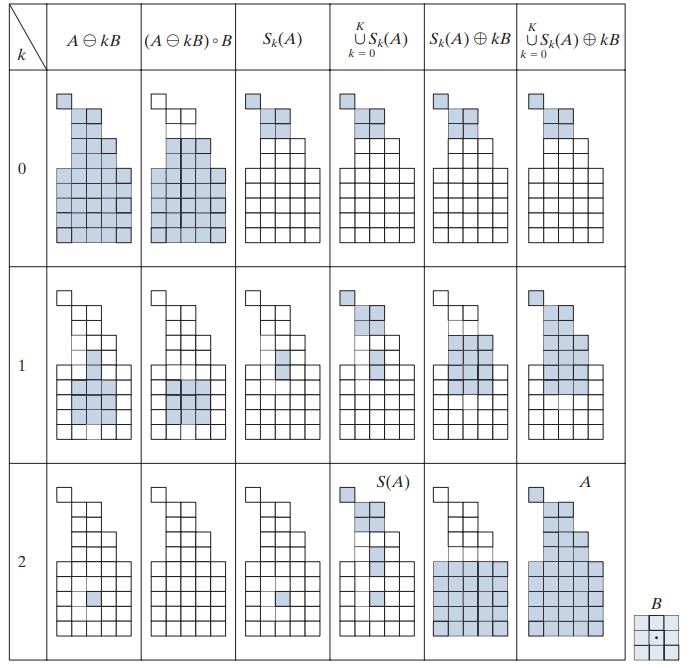
\includegraphics[width=\textwidth]{Assignment_4/output_plots/Skeleton_image_book.png}
    \caption{Image demonstrating the steps for the skeleton decomposition and reconstruction as presented in the book (fig. 9.26) \cite{gonzalez2008digital}}
    \label{fig:skeleton_book}
\end{figure}

\subsection*{(a)}
The first part of the exercise is the skeleton decomposition. The function will require a binary input image and a structuring element (SE). The structuring element for will be a 3 by 3 matrix for the purpose of this exercise. We will also assume (like in the previous exercise) that the structuring element contains the origin. The decomposition follows 4 steps that have to be done \textit{K} times each. K is the determined by how many times erosion can be applied to the input image before the image is empty (step 1 applies the erosion). The steps are as follows:

\begin{equation}\label{eq:skeleton_step1}
    A \ominus k B
\end{equation}
\begin{equation}\label{eq:skeleton_step2}
    (A \ominus k B) \circ B
\end{equation}
\begin{equation}\label{eq:skeleton_step3}
    S_k(A) = (A \ominus k B) - ((A \ominus k B) \circ B)
\end{equation}
\begin{equation}\label{eq:skeleton_step4}
    \bigcup_{k=0}^{K}S_k(A)
\end{equation}

Where: A = input image, B = structuring element, and $S_k$ = skeleton for iteration k.

The first 4 columns of Figure \ref{fig:skeleton_book} demonstrate how these four steps work for a simple binary image. The first step is applying corrosion to the input image \textit{k} times, which follows Equation \ref{eq:skeleton_step1}. In the example from the book the image would be completely empty if a corrosion was applied 3 times, so \textit{K=2}. The second step is an opening applied to the result of step 1, which follows Equation \ref{eq:skeleton_step2}. Step 3 is the skeleton for a specific \textit{k}. This is done by subtracting the result of step 2 from the result of step 1. It follows Equation \ref{eq:skeleton_step3}, which is Eq. 9-29 in the book. The fourth and final step of the decomposition is taking the union of the different skeletons $S_k$. Important to note is that for Equation \ref{eq:skeleton_step1} the erosion is applied \textit{k} times, each time taking the result of the previous iteration. This can also be written as Equation \ref{eq:erosion_k_times}, which is Eq. 9-30 in the book. Using all these steps the final skeleton is generated by taking the result of the highest \textit{k} for step 4.

\begin{equation}\label{eq:erosion_k_times}
    A \ominus k B = ((\dots((A \ominus B) \ominus B) \ominus \dots) \ominus B)
\end{equation}

The assignment requires us to implement the skeleton decomposition using a recursive function. So each level of \textit{k} should be done by a recursion and not a loop. We implemented it as such by adding the result of the current level ($S_k$) and the result of the next level together, by calling the same function again. For this we use the base case where applying erosion to the input image would result in an empty image. If this is the case the result of the current level is returned without calling the function again.

Because the result of the function would simply give the final skeleton and the different levels of the skeleton ($S_k$) could not be retrieved anymore, we need to encode the resulting images in such a way they can be retrieved. This needs to be done according to Equation \ref{eq:skeleton_encoding}, where we encode all the skeleton sets $S_k(A)$ by introducing a skeleton function \textit{skf(A)}. This basically boils down to the skeleton of each level being added to the result with a different number, namely (\textit{k+1}). Which allows us to understand the different levels of the skeleton in the reconstruction step.

\begin{equation}\label{eq:skeleton_encoding}
[\operatorname{skf}(A)](i, j)=\left\{\begin{array}{ll}
k+1, & (i, j) \in S_{k}(A) \\
0, & (i, j) \notin S_{k}(A)
\end{array}\right.
\end{equation}

The results of this function are presented in part (c) of the exercise and in Figure \ref{fig:skeleton_results}. The implementation of the function can be found in \ding{118} Listing \ref{code:IPskeletondecomp}.

\subsection*{(b)}
The next part will be the reconstruction of the skeleton we created in part (a). To reconstruct the image two steps have to be executed. Each step has to be executed \textit{k} times.

\begin{equation}\label{eq:skeleton_step5}
    S_k(A) \oplus k B
\end{equation}
\begin{equation}\label{eq:skeleton_step6}
    \bigcup_{k=0}^{K}S_k(A) \oplus k B
\end{equation}

The first step, Equation \ref{eq:skeleton_step5}, is the dilation of the skeleton for that level. The second step is the union of the results from the first step and follows Equation \ref{eq:skeleton_step6} (Eq. 9-32 in the book). The different levels of the skeleton can be distinguished as such due to the number written. The assignment requires the reconstruction to also make use of recursion instead of loops. For our implementation we extract the pixel coordinates that contain the value 1 which is the result of the first step for each \textit{k}. Afterwards we decrease all non-zero values in the remaining skeleton and apply the dilation for each number. In case certain coordinates would have multiple numbers due to the different dilations overlapping the highest number is kept. This means that the intermediate result is not correct in these cases, but the final result is correct. In the fifth column of Figure \ref{fig:skeleton_book} the entry for \textit{k=1} would not have the bottom 3 pixels, because those would be claimed by the ongoing erosion of \textit{k=2}. These intermediate levels can be correctly extracted, which we show on lines 33 to 35 in \ding{118} Listing \ref{code:IPskeletonrecon}, but are not passed to the next iteration of the recursion. We use recursion in the same way as we did for the skeleton decomposition, so we add the result of the current step and the result of a call to the same function together. The base case this time is an empty skeleton set, which means that all the skeleton sets have been processed.

The results of this function are presented in part (c) of the exercise and in Figure \ref{fig:skeleton_results}. The implementation of the function can be found in \ding{118} Listing \ref{code:IPskeletonrecon}.

\subsection*{(c)}
The last part of the assignment requires us to show the results of our implementation of the skeleton decomposition and reconstruction using the input image \textit{nutsbolts.tif}. In Figure \ref{fig:skeleton_results} the input image, the reconstructed image, the skeleton, and the difference between the input image and reconstructed image are shown. The difference image is completely back, meaning that the reconstruction is a perfect match for the input image. This is also verified by taking the absolute difference of the two images in the code.

To demonstrate our implementations we created a test file that generates the skeleton and reconstruction images, this can be found in \ding{118} Listing \ref{code:IPskeleton_test}.

\begin{figure}[H]
     \centering
     \begin{subfigure}[t]{0.49\textwidth}
         \centering
         \includesvg[width=\textwidth]{Assignment_4/output_plots/skeleton_input.svg}
         \caption{The \textit{nutsbolts.tif} input image (saved as an svg)}
         \label{fig:skeleton_input}
     \end{subfigure}
     \hfill
     \begin{subfigure}[t]{0.49\textwidth}
         \centering
         \includesvg[width=\textwidth]{Assignment_4/output_plots/skeleton_reconstruction.svg}
         \caption{The reconstruction of the image. This is the produced by passing the result of \textit{IPskeletondecomp} to the \textit{IPskeletonrecon} function.}
         \label{fig:skeleton_reconstruction}
     \end{subfigure}
     \newline
     \begin{subfigure}[t]{0.49\textwidth}
         \centering
         \includesvg[width=\textwidth]{Assignment_4/output_plots/skeleton_skeleton.svg}
         \caption{The complete skeleton image. This is produced by passing the binary input image \ref{fig:skeleton_input} to the \textit{IPskeletondecomp} function.}
         \label{fig:skeleton_skeleton}
     \end{subfigure}
     \hfill
     \begin{subfigure}[t]{0.49\textwidth}
         \centering
         \includesvg[width=\textwidth]{Assignment_4/output_plots/skeleton_difference.svg}
         \caption{The difference image of the input image and the reconstructed image. The absolute difference is 0 here (this is verified in the code, see \ding{118} Listing \ref{code:IPskeleton_test}), meaning the images are exactly the same and this image is completely black.}
         \label{fig:skeleton_difference}
     \end{subfigure}
    \caption{The results from applying our implementation of skeleton decomposition and reconstruction to the input image \textit{nutsbolts.tif}.}
    \label{fig:skeleton_results}
\end{figure}

\section*{Individual contributions}
\begin{itemize}
    \item \textbf{Exercise 1 and 2}. Contribution to program design, program implementation, answering questions posed and writing the report: \textit{Jeroen} 100\%.
    \item \textbf{Exercise 3}. Contribution to program design, program implementation, answering questions posed and writing the report: \textit{Kevin} 100\%.
\end{itemize}

\bibliographystyle{plain}
\typeout{}
\bibliography{Assignment_4}

\newpage
\appendix
\section{Code}
\subsection{Exercise 2}
\lstinputlisting[caption={IPmorph.m: perform morphological transformations, namely \textit{dilation} and \textit{erosion}, using a single function.}, label={code:IPmorph}]{Assignment_4/IPmorph.m}

\subsubsection{Exercise 2 (a)}
\lstinputlisting[caption={\texttt{IPdilate.m}: perform dilation using \textsc{IPmorph} (Listing~\ref{code:IPmorph}).}, label={code:IPdilate}]{Assignment_4/IPdilate.m}
\subsubsection{Exercise 2 (b)}
\lstinputlisting[caption={\texttt{IPerode.m}: perform dilation using \textsc{IPmorph} (Listing~\ref{code:IPmorph}).}, label={code:IPerode}]{Assignment_4/IPerode.m}
\subsubsection{Exercise 2 (c)}
\lstinputlisting[caption={\texttt{IPdilate\_erode\_test.m}: Test script to demonstrate the functionality of both \textsc{IPdilate} and \textsc{IPerode}. Saves images to .svg files.}, label={code:IPdilate_erode_test}]{Assignment_4/IPdilate_erode_test.m}

\subsection{Exercise 3}
\subsubsection{Exercise 3 (a)}
\lstinputlisting[caption={\texttt{IPskeletondecomp.m}: Perform skeleton decomposition of the binary input image.}, label={code:IPskeletondecomp}]{Assignment_4/IPskeletondecomp.m}
\subsubsection{Exercise 3 (b)}
\lstinputlisting[caption={\texttt{IPskeletonrecon.m}: Perferm image reconstruction using the skeleton.}, label={code:IPskeletonrecon}]{Assignment_4/IPskeletonrecon.m}
\subsubsection{Exercise 3 (c)}
\lstinputlisting[caption={\texttt{IPskeleton\_test.m}: Test script to demonstrate the functionality of both \textsc{IPskeletondecomp} and \textsc{IPskeletonrecon}.}, label={code:IPskeleton_test}]{Assignment_4/IPskeleton_test.m}
\end{document}
